

\subsection{Symbolic Coordinates and User Transformations}
\label{pgfplots:sec:symbolic:coords}
\PGFPlots\ supports user transformations which can be applied to input and output coordinates. Suppose the plot shall display days versus account statements over time. Then, one wants to visualize date versus credit balance. But: dates need to be transformed to numbers before doing so! Furthermore, tick labels shall be displayed as dates as well. This, and more general transformations, can be realized using the |x coord trafo| and |y coord trafo| keys.

\paragraph{Remark:} This section applies to users who want to have non-standard input \emph{coordinates}. If you have normal numbers which don't need to be transformed and you like to have special symbols as tick labels, you should consider using the \declaretext{[xyz]ticklabels} key described on page~\pageref{pgfplots:key:xticklabels}.

\begin{pgfplotsxycodekeylist}{
	\x\ coord trafo,
	\x\ coord inv trafo}
	These code keys allow arbitrary coordinate transformations which are applied to input coordinates and output tick labels.

	The |x coord trafo| and |y coord trafo| command keys take one argument which is the input coordinate. They are expected to set |\pgfmathresult| to the final value.

	At this level, the input coordinate is provided as it is found in the |\addplot| statement. For example, if $x$ coordinates are actually of the form \meta{year}-\meta{month}-\meta{day}, for example |2008-01-05|, then a useful coordinate transformation would transform this string into a number (see below for a predefined realization).

	In short, \emph{no} numerics has been applied to input coordinates when this transformation is applied\footnote{Of course, if coordinates have been generated by gnuplot or \pgfname, this does no longer hold.}.

	The input coordinate transformation is applied to
	\begin{itemize}
		\item any input coordinates (specified with |\addplot| or |axis cs|),
		\item any user-specified |xtick| or |ytick| options,
		\item any user-specified |extra x ticks| and |extra y ticks| options,
		\item any user-specified axis limits like |xmin| and |xmax|.
	\end{itemize}

	The output coordinate transformation |x coord inv trafo| is applied to tick positions just before evaluating the |xticklabel| and |yticklabel| keys. The argument to |x coord inv trafo| is a fixed point number (which may have trailing zeros after the period).
	The tick label code may use additional macros defined by the inverse transformation.

	Remark: \PGFPlots\ will continue to produce tick positions as usual, no extra magic is applied. It may be necessary to provide tick positions explicitly if the default doesn't respect the coordinate space properly.

	The initial value of these keys is
\begin{codeexample}[code only]
\pgfplotsset{
	x coord trafo/.code={},
	x coord inv trafo/.code={}}
\end{codeexample}
	\noindent which simply disables the transformation (the same for $y$, of course).

	\paragraph{Remark:} It might be necessary to set
\begin{codeexample}[code only]
\pgfplotsset{
	/pgfplots/xticklabel={\tick},
	/pgfplots/scaled x ticks=false
}
\end{codeexample}
	\noindent in order to avoid number formatting routines on |\tick| or numerics for tick scale methods. This is done automatically by the predefined symbolic coordinate styles (see below).
\end{pgfplotsxycodekeylist}

\subsubsection{String Symbols as Input Coordinates}
It is possible to provide a string dictionary to \PGFPlots. An input coordinate can then use any symbol provided in that dictionary.
\begin{pgfplotsxykeylist}{symbolic \x\space coords=\marg{dictionary}}%
	A styles which sets |x coord trafo| and |x coord inv trafo| (or the respective |y| or |z| variants) such that any element in \marg{dictionary} is a valid input coordinate. The \marg{dictionary} can be a comma separated list or a list terminated with `|\\|'. In both case, white spaces are considered to be part of the names (use `|%|' at end of lines).

	The dictionary will assign integer numbers to every element. These integers are used internally for arithmetics. Finally, the inverse transformation takes a fixed point number and maps it to the nearest integer, and that integer is mapped into the dictionary.
\begin{codeexample}[]
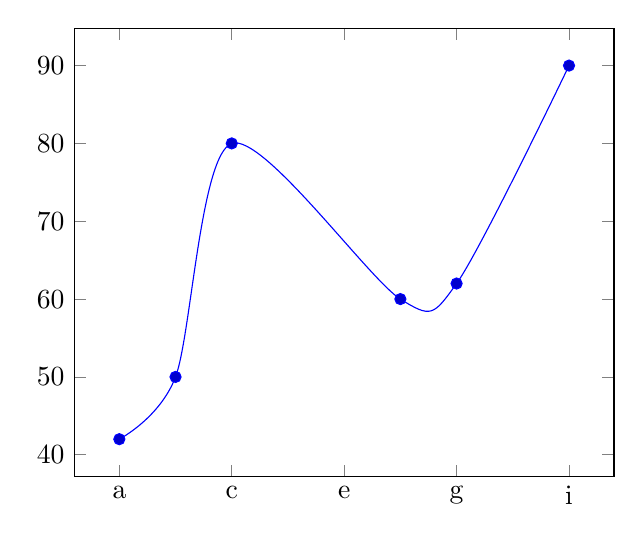
\begin{tikzpicture}
\begin{axis}[symbolic x coords={a,b,c,d,e,f,g,h,i}]
	\addplot+[smooth] coordinates {
		(a,42)
		(b,50)
		(c,80)
		(f,60)
		(g,62)
		(i,90)};
\end{axis}
\end{tikzpicture}
\end{codeexample}
	
	The effect of the transformation is simply that input coordinates can be elements of the dictionary and tick labels will be chosen out of this dictionary as well.
\end{pgfplotsxykeylist}

\subsubsection{Dates as Input Coordinates}
\label{pgfplots:sec:date:coords}
The already mentioned application of using dates as input coordinates has been predefined, together with support for hours and minutes. It relies on the \pgfname\ calendar library which converts dates to numbers in the julian calendar. Then, one coordinate unit is one day.

\begin{pgfplotslibrary}{dateplot}
	Loads the coordinate transformation code.
\end{pgfplotslibrary}

\begin{stylekey}{/pgfplots/date coordinates in=\mchoice{x,y}}
	Installs |x coord trafo| and |x coord inv trafo| (or the respective $y$ variant) such that ISO dates of the form \meta{year}|-|\meta{month}|-|\meta{day} are accepted. For example, |2006-02-28| will be converted to an ``appropriate'' integer using the julian calender. Input coordinates may be of the form
		
		\meta{year}|-|\meta{month}|-|\meta{day}

	\noindent or they may contain times as

		\meta{year}|-|\meta{month}|-|\meta{day} \meta{hour}|:|\meta{minute}.

	The result of the transformation are numbers where one unit is one day and times are fractional numbers.

	The transformation is realized using the \pgfname-calendar module, see \cite[Calendar Library]{tikz}. This reference also contains more information about extended syntax options for dates.

	The inverse transformation provides the following macros which are available during tick label evaluation (i.e. when used inside of |xticklabel| or |yticklabel|):
	\begin{itemize}
		\item |\year| expands to the year component,
		\item |\month| expands to the month component,
		\item |\day| expands to the day component,
		\item |\hour| expands to the hour component (using two digits),
		\item |\Hour| expands to the hour component (but omits leading zeros),
		\item |\minute| expands to the minute component (two digits),
		\item |\Minute| expands to the minute component (omits leadings zeros),
		\item |\lowlevel| expands to the low level number representing the tick,
		\item |\second| will always be |00|.
	\end{itemize}
	This allows to use |\day.\month.\year| or |\day. \hour:\minute| inside of |xticklabel|, for example.

	A complete example (with fictional data) is shown below.
\pgfplotsset{anchor=center,/tikz/every picture/.append style={baseline}}
% \usepgfplotslibrary{dateplot}\usepackage{eurosym}
\begin{codeexample}[]
% requires \usepgfplotslibrary{dateplot} !

\pgfplotstabletypeset[string type]{plotdata/accounts.dat}

\begin{tikzpicture}
	\begin{axis}[
		date coordinates in=x,
		xticklabel={\day.\month.},
		xlabel={2008},
		stack plots=y,
		yticklabel={\pgfmathprintnumber{\tick}\EUR{}}, % <- requires \usepackage{eurosym}
		ylabel=Total credit,
		ylabel style={yshift=10pt},
		legend style={
			at={(0.5,-0.3)},anchor=north,legend columns=-1}]
		
	\addplot table[x=date,y=account1] {plotdata/accounts.dat};
	\addplot table[x=date,y=account2] {plotdata/accounts.dat};
	\addplot table[x=date,y=account3] {plotdata/accounts.dat};
	\legend{Giro,Tagesgeld,Sparbuch}
	\end{axis}
\end{tikzpicture}
\end{codeexample}

% \usepgfplotslibrary{dateplot}\usepackage{eurosym}
\begin{codeexample}[]
% requires \usepgfplotslibrary{dateplot} !
\begin{tikzpicture}
  \begin{axis}[
    date coordinates in=x,
    xtick=data,
    xticklabel style=
		{rotate=90,anchor=near xticklabel},
    xticklabel=\day. \hour:\minute,
    date ZERO=2009-08-18,% <- improves precision!
  ]
  \addplot coordinates {
    (2009-08-18 09:00,  050)
    (2009-08-18 12:00,  100)
    (2009-08-18 15:00,  100)
    (2009-08-18 18:35,  100)
    (2009-08-18 21:30,  040)
    (2009-08-19,        020)
    (2009-08-19 3:00,   000)
    (2009-08-19 6:0,    035)
  };
  \end{axis}
\end{tikzpicture}
\end{codeexample}

\paragraph{Attention:} If you intend to use hours and minutes, you should \emph{always} provide the |date ZERO| to maintain adequate precision!
\end{stylekey}

\begin{pgfplotskey}{date ZERO=\meta{year}-\meta{month}-\meta{day} (initially 2006-01-01)}
	A technical key which defines the $0$ coordinate of |date coordinates in|. Users will never see the resulting numbers, so one probably never needs to change it. However, the resulting numbers may become very large and a mantisse of 6 significant digits may not be enough to get accurate results. In this case, |date ZERO| should be set to a number which falls into the input date range.
\end{pgfplotskey}
